\documentclass[10pt,a4paper]{article}
\usepackage[utf8]{inputenc}
\usepackage[english]{babel}
%\usepackage[OT1]{fontenc}
\usepackage{amsmath}
%\usepackage{amsfonts}
\usepackage{amssymb}
\usepackage[left=20mm,right=20mm, top=20mm,bottom=15mm,bindingoffset=0cm]{geometry}


\usepackage[T1]{fontenc}
\usepackage{graphicx}
%\usepackage{lmodern}

\title{Optimal P2P network}
\author{Nikita Popov, Danil Kharasov, Yaroslav Kishchenko}
\begin{document}
\maketitle
\section*{Problem description}

Suppose we have a network of $N$ computers, and one of them (or several) has a file that we want to distribute to every other peer. The sooner all the computers will have the file the better, and this is the optimization task we want to solve. 

Our base model for this task will be continuous, and later we will discretize the problem. Connections between peers can be modelled via graph: vertices of the graph will represent the computers in our network, and weights of the edges is the bandwidth between the pair of the computers. Let the adjacency matrix of this graph be $B$. Besides the bandwidth of pairs we also have connection speed of every computer to the network. This values will be assigned to vertices. Let $u_i$ be maximum upload speed for the computer $i$, and $d_i$ be the maximum download speed for the computer $i$. 

The last part of our model (and the beginning of discretization) is the file description. All we need to now is file's length, we will name it $L$. We will split the file in $K$ parts and will deliver the parts along the net. Discretizing time and recomputing the bandwidth and all upload and download restrictions in terms of amount of parts (which will be integers),

\begin{equation}
	\hat{b}_{ij} = b_{ij} \frac{dt}{dL}
\end{equation}
where $dL = \frac{L}{K}, dt$ -- time step, we now ready to formulate the problem.

Let $x_{ikt}$ be a variable that is equals to $1$ when computer $i$ has a part $k$ at the moment of time $t$ and to $0$ otherwise, and $y_{ijkt}$ be a variable that is equals to $1$ when part $k$ was transferred from computer $i$ to computer $j$ at moment of time $t$. In terms of $x$ and $y$ we want to minimize the following thing:
\begin{equation}
	\max_{i} \min \{t: \sum_k x_{ikt} = K \} \to \min_{x, y}.
\end{equation} 

In other words, we want to minimize the time when all computers in network will have all parts of the file. Now let's formulate the restrictions on the variables $x, y$:
\begin{align}
	\label{bandwidth}	\sum_k y_{ijkt} \leqslant & \ b_{ij} \\ 
	\label{download}	\sum_{ik} y_{ijkt} \leqslant & \ d_j \\ 
	\label{upload}	\sum_{jk} y_{ijkt} \leqslant & \ u_i \\ 
	\label{nonerasability}	\forall t' \geqslant t \  x_{ikt'} \geqslant & \ x_{ikt} \\ 
	\label{availability}	y_{ijkt} \leqslant & \ x_{ikt} \\
	\label{piece_available} y_{ijkt} \leqslant & \ x_{jk,t+1} \\
	\label{piece_downloaded} \sum\limits_{i,t} y_{ijkt} = & \ 1 \\
	\label{starting_conditions} \forall i \in S_0 \ x_{ik0} = 1, & \forall i \notin S_0 \ x_{ik0} = 0 \\
	\label{binary} x_{ikt}, y_{ijkt} \in & \ \{0, 1 \}.
\end{align}

The description of every inequality is the following:
\begin{itemize}
	\item Equation \eqref{bandwidth} is the bound on the amount of parts that can be transferred within connection between $i$ and $j$.
	\item Equations \eqref{download} and \eqref{upload} restrict the uploads and downloads for computer $i$.
	\item Equations \eqref{nonerasability} forbid the disappearance of the part $k$ from computer $i$.
	\item Equations \eqref{availability} state that part $k$ can be downloaded from computer $i$ if and only if this part has been downloaded to the computer $i$ before.
	\item Equation \eqref{piece_available} make the piece $k$ available on computer $j$ in next time step.
	\item Equations \eqref{piece_downloaded} forces the file piece to be downloaded from only one source in only one moment of time.
	\item Equations \eqref{starting_conditions} imply that computers $S_0$ have the whole file at the beginning.
	\item Equations \eqref{binary} requires the $x$ and $y$ to be binary.
\end{itemize}

Every restriction is linear in terms of $x$ and $y$. To finalize this problem as a linear programming problem, we need to reduce the objective to a linear form. We use the following expression:
\begin{equation}
	\max_{i} \min \{t: \sum_k x_{ikt} = K \} \to \min_{x,y} \Rightarrow \max_i \sum_t \gamma_t\Big( K - \sum_k x_{ikt} \Big) \to \min_{x, y},
\end{equation}
where $\gamma_t$ are just increasing weights to force optimizer switch $x$'s to ones as soon as possible.

First of all, it is not the same objective, but it's close: when computer $i$ downloaded file, the expression $K - \sum_k x_{ikt}$ tends to zero, so the sooner the the computer download the file the better, but not in the same way better. Still, it's close. And the part $\sum_t \gamma_t K$ is constant, so we will minimize $\max_i \sum_{kt} x_{ikt}$.

This is the final problem:
\begin{align*}
	\begin{array}{rrll}
	& \min\limits_{x, y, \xi} \xi \\ 
	\ \\
	& \sum\limits_k y_{ijkt} \leqslant & \mkern-12mu b_{ij} \\ 
	& \sum\limits_{ik} y_{ijkt} \leqslant & \mkern-12mu d_j \\ 
	& \sum\limits_{jk} y_{ijkt} \leqslant & \mkern-12mu u_i \\ 
	& x_{ikt'} \geqslant & \mkern-12mu x_{ikt} & \mkern-32mu \forall t' \geqslant t  \\ 
	s. t. & y_{ijkt} \leqslant & \mkern-12mu x_{ikt} \\
	& y_{ijkt} \leqslant & \mkern-12mu x_{jk,t+1} \\
	& \sum\limits_{i,t} y_{ijkt} = & \mkern-12mu 1 \\
	& \forall i \in S_0 \ x_{ik0} = & \mkern-12mu 1 \\
	& \forall i \notin S_0 \ x_{ik0} = & \mkern-12mu 0 \\	
	& x_{ikt}, y_{ijkt} \in & \mkern-12mu \{0, 1 \} \\
	& -\sum\limits_{kt} x_{ikt} \leqslant & \mkern-12mu \xi & \mkern-50mu \forall i
	\end{array} 
\end{align*}
Variable $\xi$ imitates the maximum.

\section*{Data generation}
We generate data as following: first, we randomly generate positions on a plane for each computer and it's connection type (ADSL, Ethernet or Dial-Up). Then, we create a bandwidth matrix as following:
\begin{equation}
	b_{ij} =  \frac{C}{\|r_i - r_j \|} \cdot ( 0.5 + R[0;0.5]),
\end{equation}
where $C$ is normalization constant, $R[a, b]$ - uniform distribution on $[a, b]$. Uniform distribution simulates connection jams between computers.

\pagebreak

\section*{Applied methods}

We tried Simplex method on relaxed problem with depth-first search of integer solution, convex optimization methods via CVXPY and greedy algorithm.

\subsection*{Greedy algorithm}
The first approach was to implement any kind of greedy algorithm. In our case we start from the fastest connections and distribute them first, and later start distributing in descending by speed connection order. 

\subsection*{CVXPY}
Unfortunately, we haven't managed to make it work - optimizer failed every our attempt stating that our problem is infeasible. But code is still in the attachments.

\subsection*{Simplex method}
The most promising method turns out to be Simplex method, but not without limitations - matrix of restrictions is huge and doesn't fit into memory for large parameters. But still, we achieved some results.

\section*{Time comparison}
\begin{table}[h]
\begin{center}
	\begin{tabular}{|c|l|l|}
		\hline 3,5,5         & 16s & 163ms \\
		\hline 4, 5, 5       & 32s & 310ms \\
		\hline 5, 5, 5       & -   & 252ms \\
		\hline 10, 10, 10    & -   & 310ms \\
		\hline 100, 100, 100 & -   &        \\
		\hline 
	\end{tabular}
	\caption{Time comparison of Simplex algorithm and greedy algorithm}
\end{center}
\end{table}

\section*{Results visualisation}

Down below reader can find visualisation for implemented algorithms. Plot means the following: axis x is for file pieces, axis y - computers. If the square is red, then this piece is downloaded on chosen computer. There are several time stamps for different situations.

\begin{figure}
	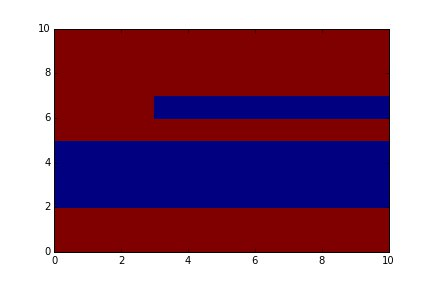
\includegraphics[scale=0.5]{pics/001} 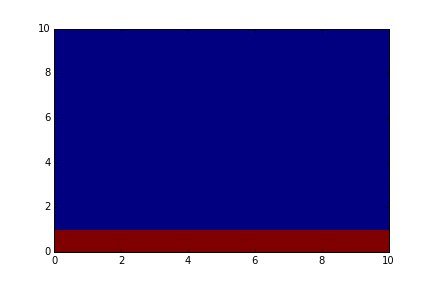
\includegraphics[scale=0.5]{pics/008} \\
	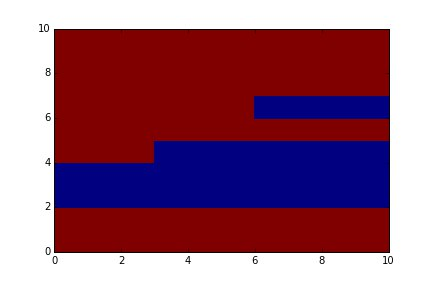
\includegraphics[scale=0.5]{pics/002} 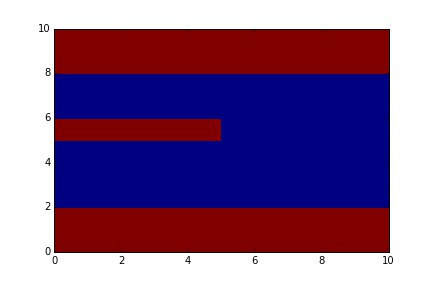
\includegraphics[scale=0.5]{pics/009} \\
	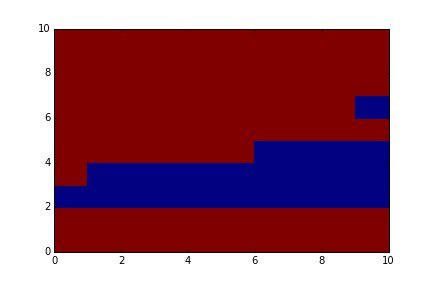
\includegraphics[scale=0.5]{pics/003} 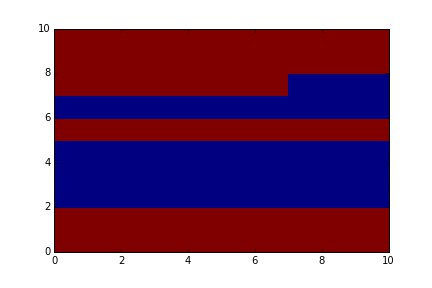
\includegraphics[scale=0.5]{pics/010} \\
	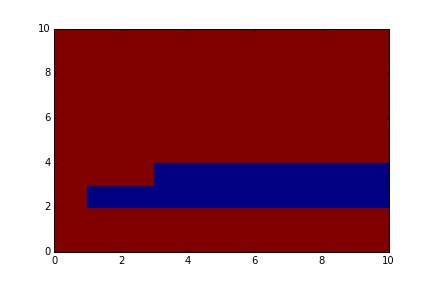
\includegraphics[scale=0.5]{pics/004}  \\
	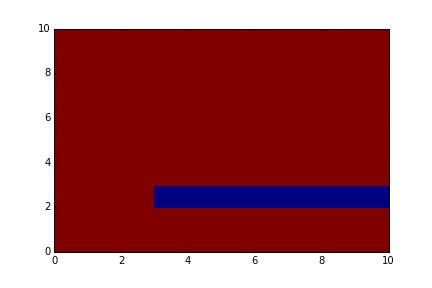
\includegraphics[scale=0.5]{pics/005} \\
	\caption{Simulation of greedy algorithm with $N = 10$ computers, $10$ file pieces for two situations}
\end{figure}

\begin{figure}
\begin{center}
	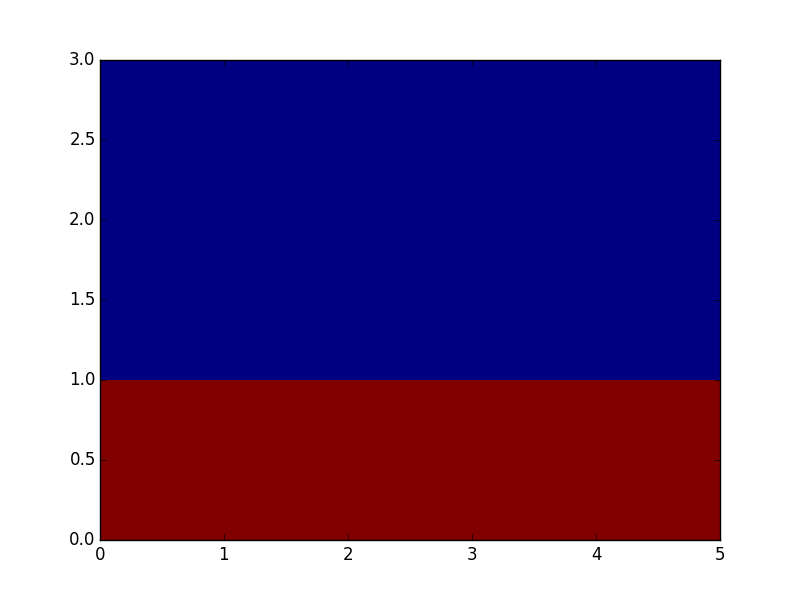
\includegraphics[scale=0.5]{sim0} \\
	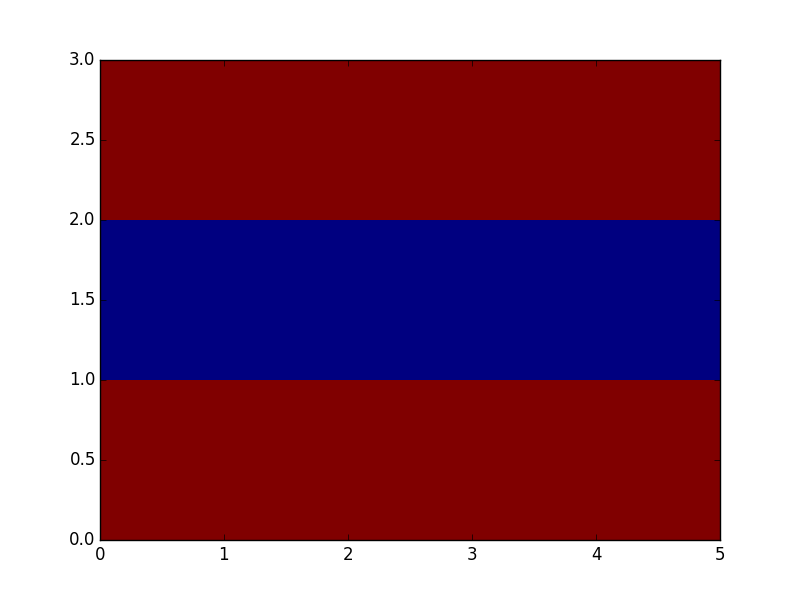
\includegraphics[scale=0.5]{sim1} \\
	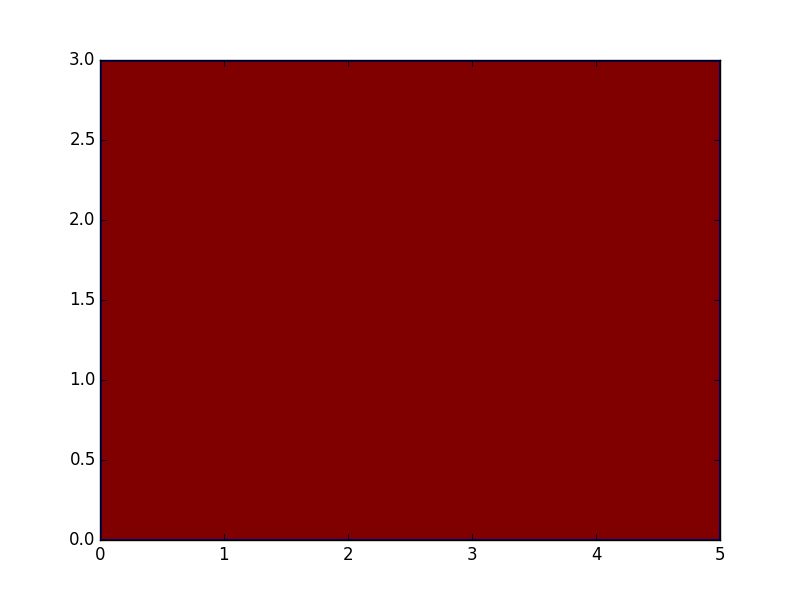
\includegraphics[scale=0.5]{sim2} \\
\end{center}
	\caption{Simulation of Simplex method with $N = 3$ computers, $5$ file pieces}
\end{figure}
\end{document}